\chapter{Discussion}

    \section{Implications for Touch Input Technology}
    Our results showed that the hand palm was the most favorite area for users to perform \emph{touch} inputs on. Half of the game inputs with \emph{touch} input used a finger to perform a gesture on the palm (See Figure \ref{fig:figureOnBodyPorpotion}). According to the mental model mentioned above, users utilized the metaphor of a trackpad and a touch-screen on the palm in several cases. Since this metaphor leads to the same input actions as on trackpads and touch-screens, current gesture interpreting algorithms like Dollar N\cite{DollarN} could be employed here.




  \begin{figure}
  \centering
  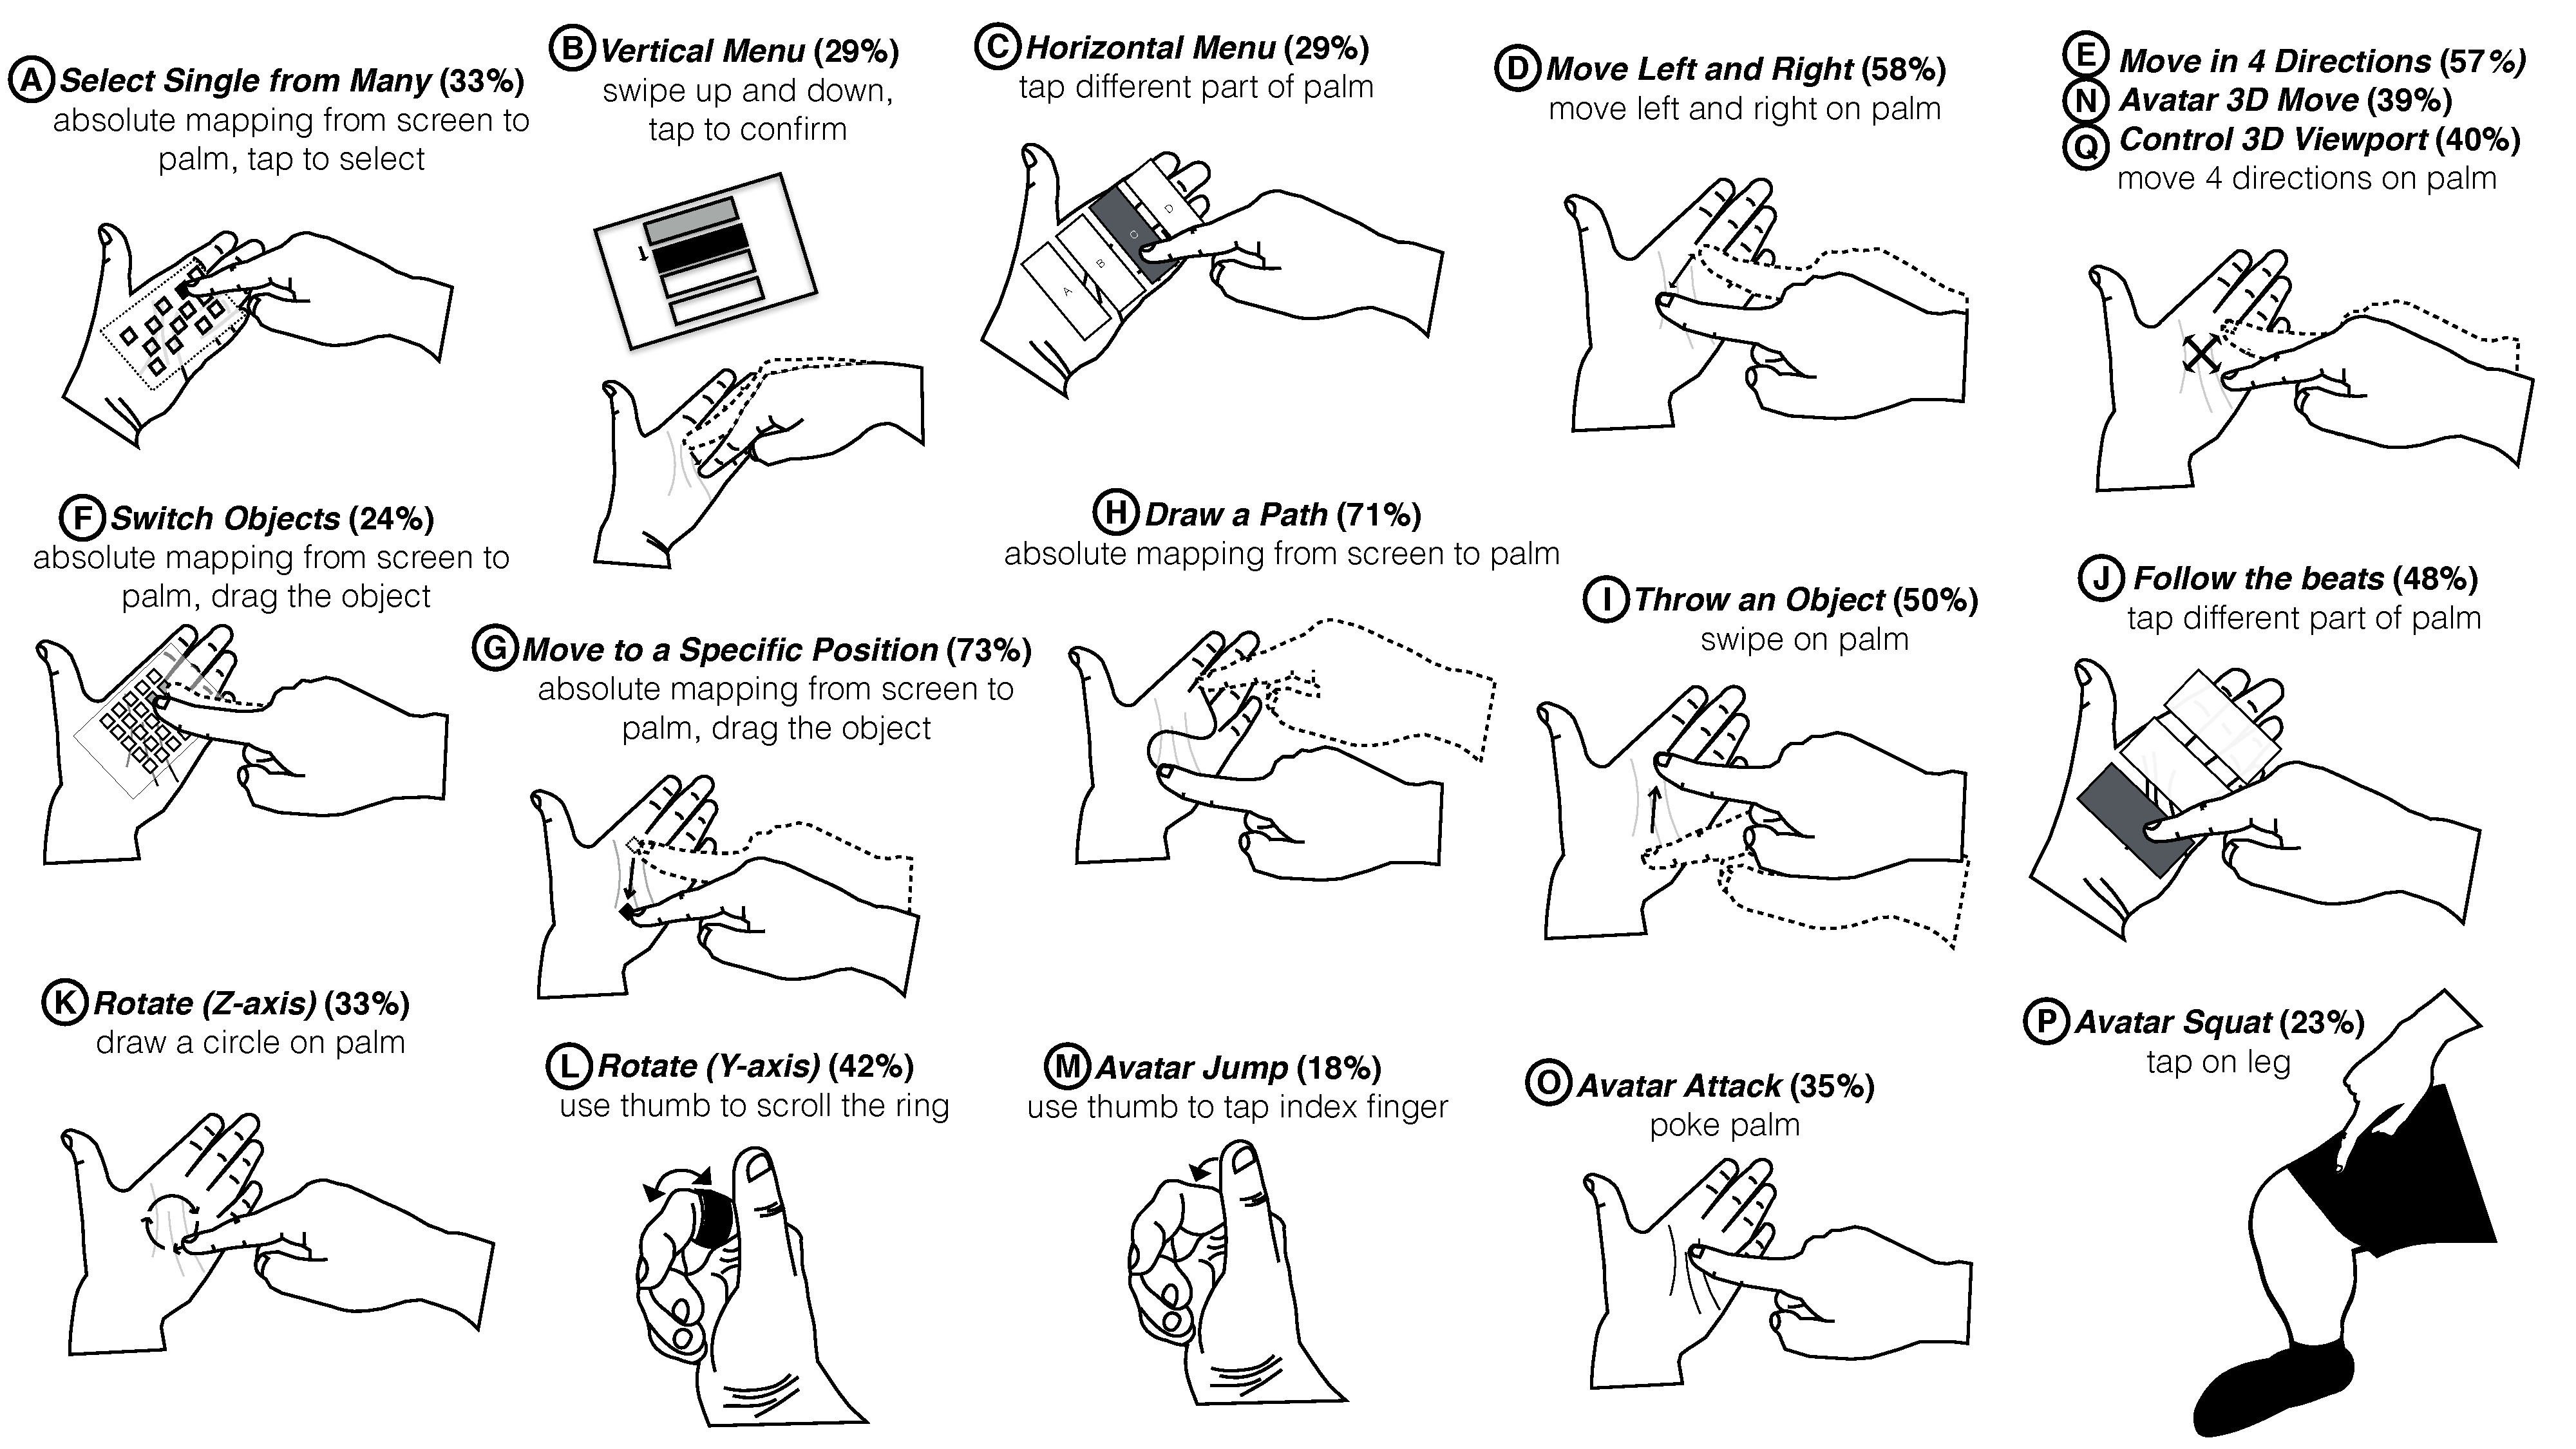
\includegraphics[width=1\textwidth]{Figures/OnBodyInputSet}
  \caption{The user-defined game input set with \emph{touch} inputs. The percentages indicate the portion of users who performed the pictured input action for the game task. Note that, there are 3 tasks (``Move in 4 directions'', ``Avatar 3D Move'', and ``Control 3D viewport'') have been assigned with an identical input action.}
  \label{fig:OnBodyInputSet}
  \end{figure}

  \begin{figure}
  \centering
  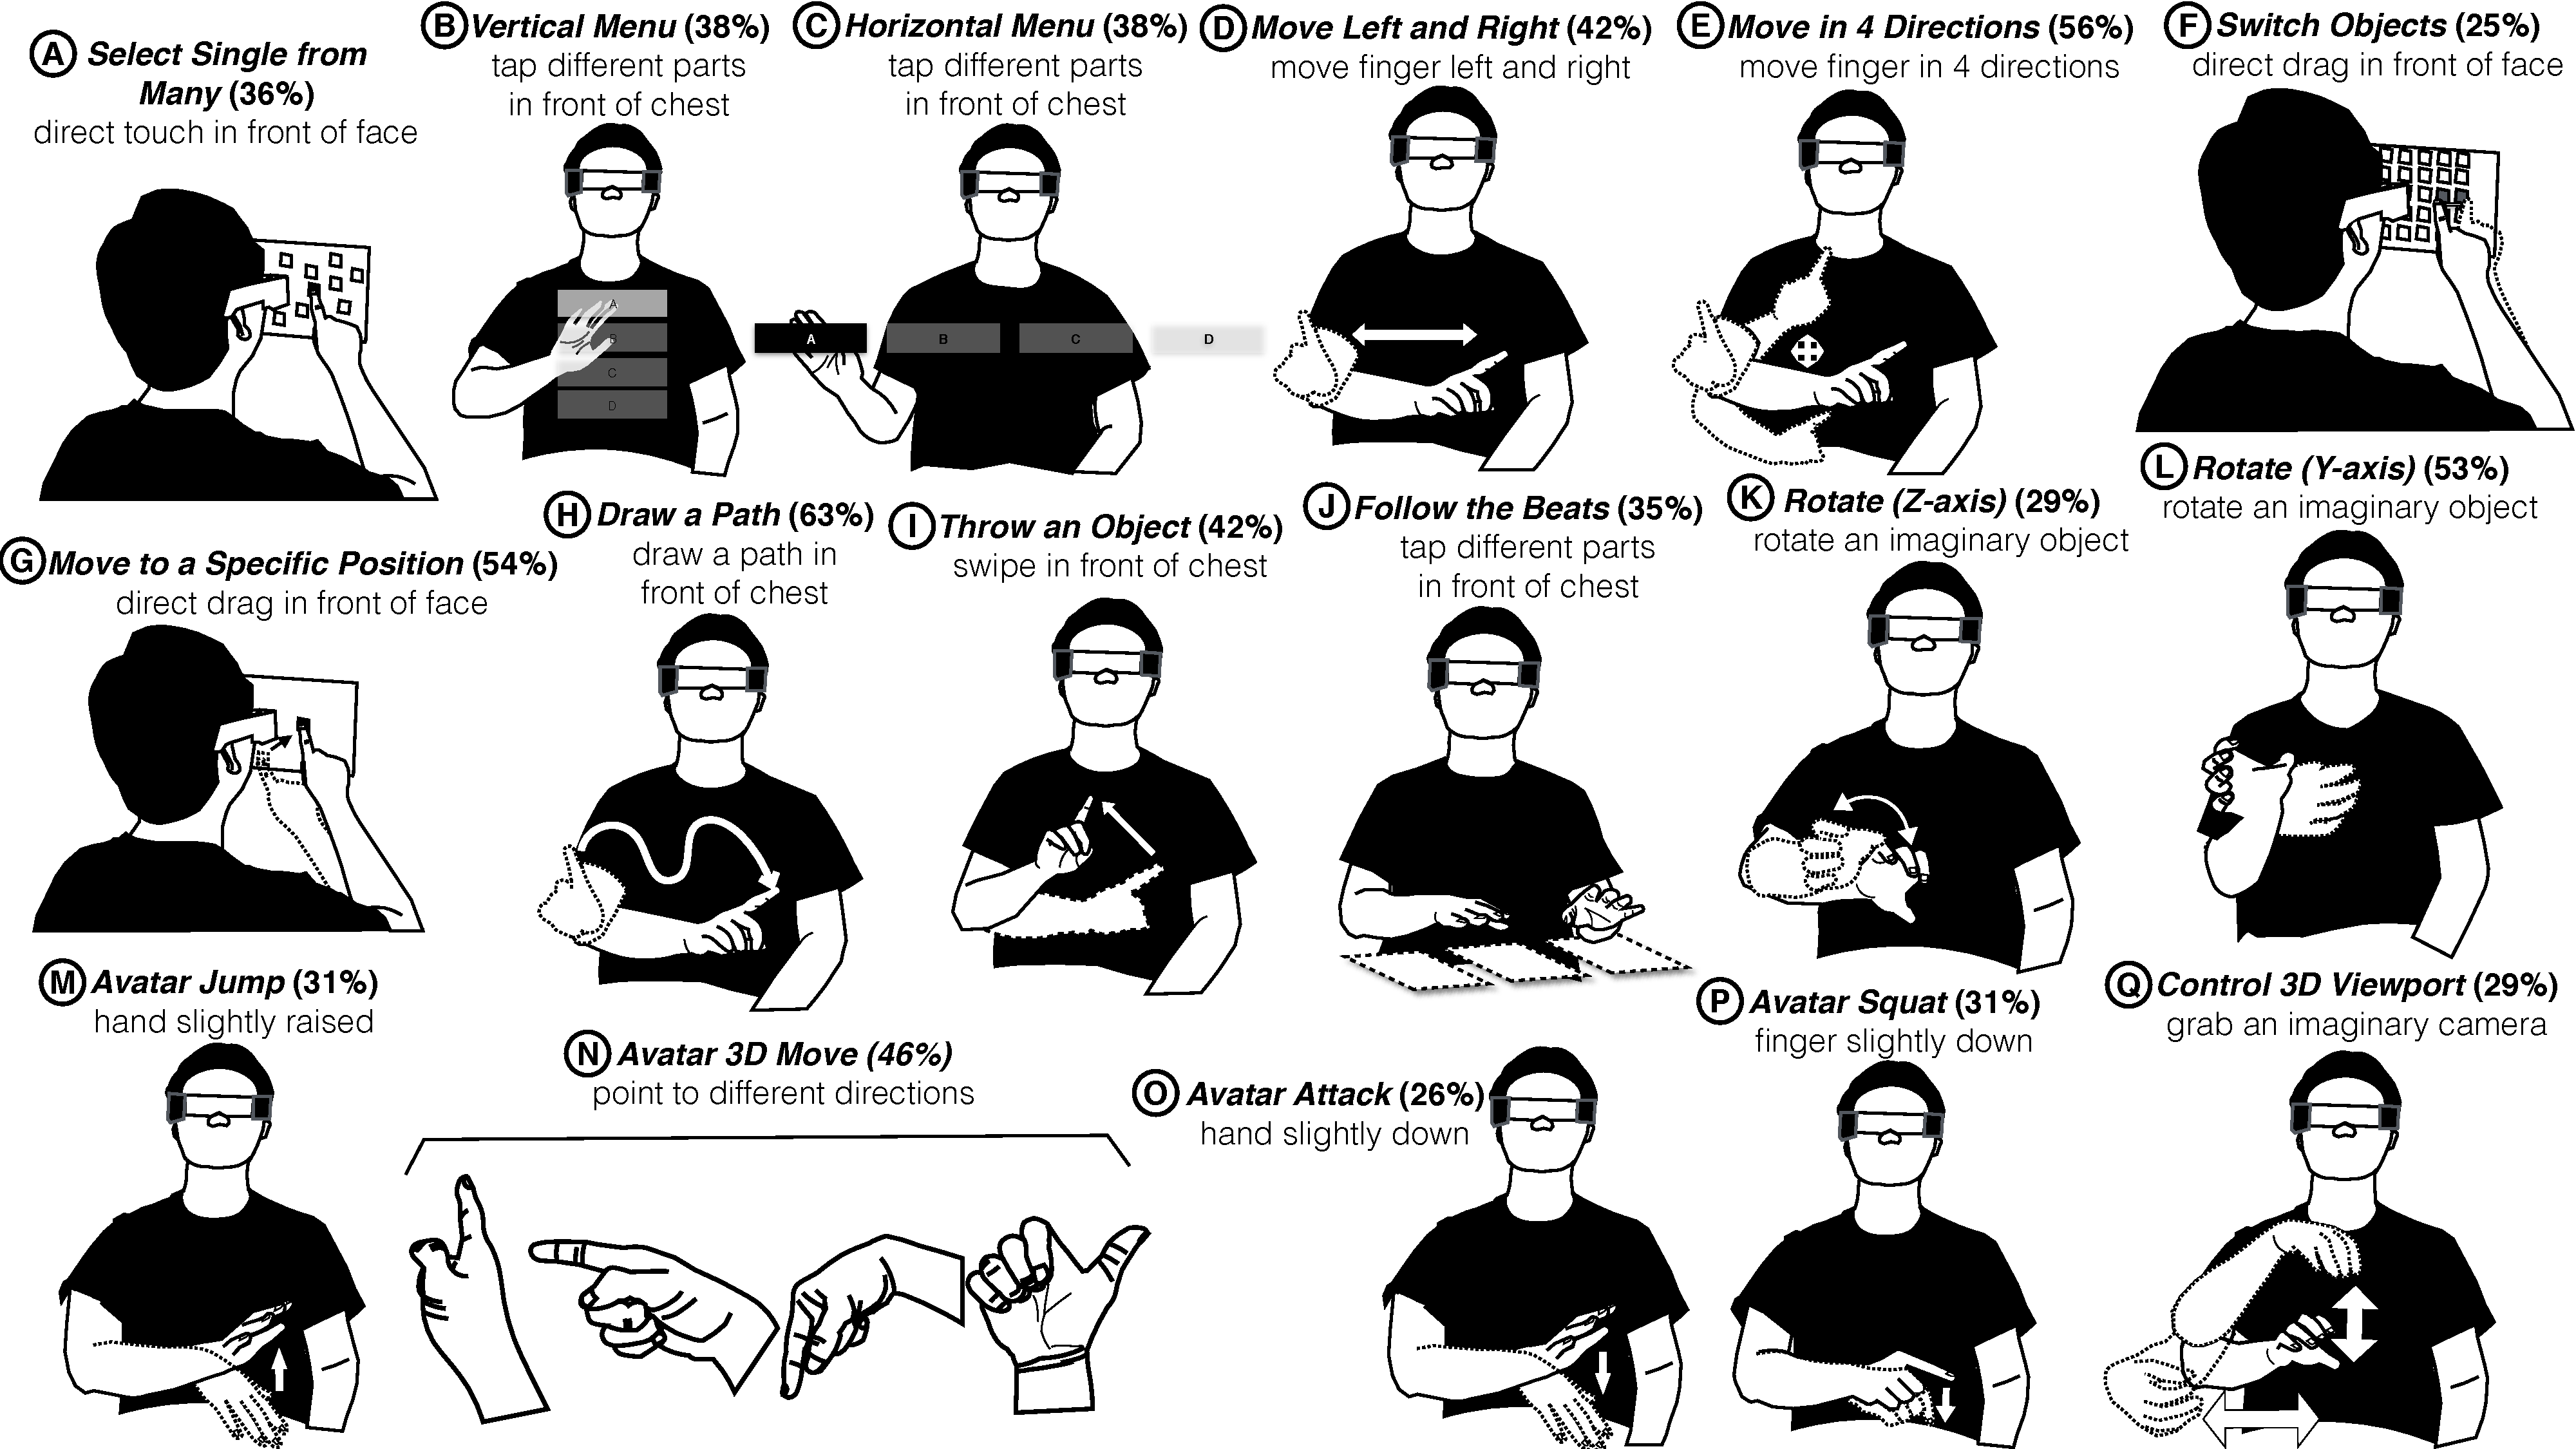
\includegraphics[width=1\textwidth]{Figures/InAirSet}
  \caption{The user-defined game input set with \emph{non-touch} interaction, The percentages indicate the portion of users who performed the pictured input action for the game task.}
  \label{fig:InAirSet}
  \end{figure}

    \section{Implications for Non-Touch Interaction Technology}
    For \emph{non-touch} interaction methods, our taxonomy shows that performing in-air gestures with fingers and hands are still the dominant forms for smart glass gaming (Figure \ref{fig:figureInAirPorpotion}.1\{A,B\}). There was only a small number of participants that used head-gestures, eye-gestures or voice controls, 7\%, 3\% and 1\% respectively.
    Before our study, both Google Glass and Mime\cite{GoogleGlass, Colaco:2013:MCL:2501988.2502042} supplied their own in-air gesture sets to increase the diversity of their input. However, our results show that 63\% of the in-air gestures are not performed in front of the user's face in the public space due to the social acceptance issues and physical tiring problems mentioned before (see Figure \ref{fig:figureInAirPorpotion}.2). Therefore, if the developers of head-worn devices want to implement in-air gestures for input, they will need to have the capability to sense gestures in a wide range of areas near the user other than only right in front of the face. Take CV-based sensing technologies for example, instead of a regular lens, we could use a wide-angle lens or fish-eye lens to implement a system to cater to the user's preference \cite{Chan:2015}.
  \begin{figure}[!h]
  \centering
  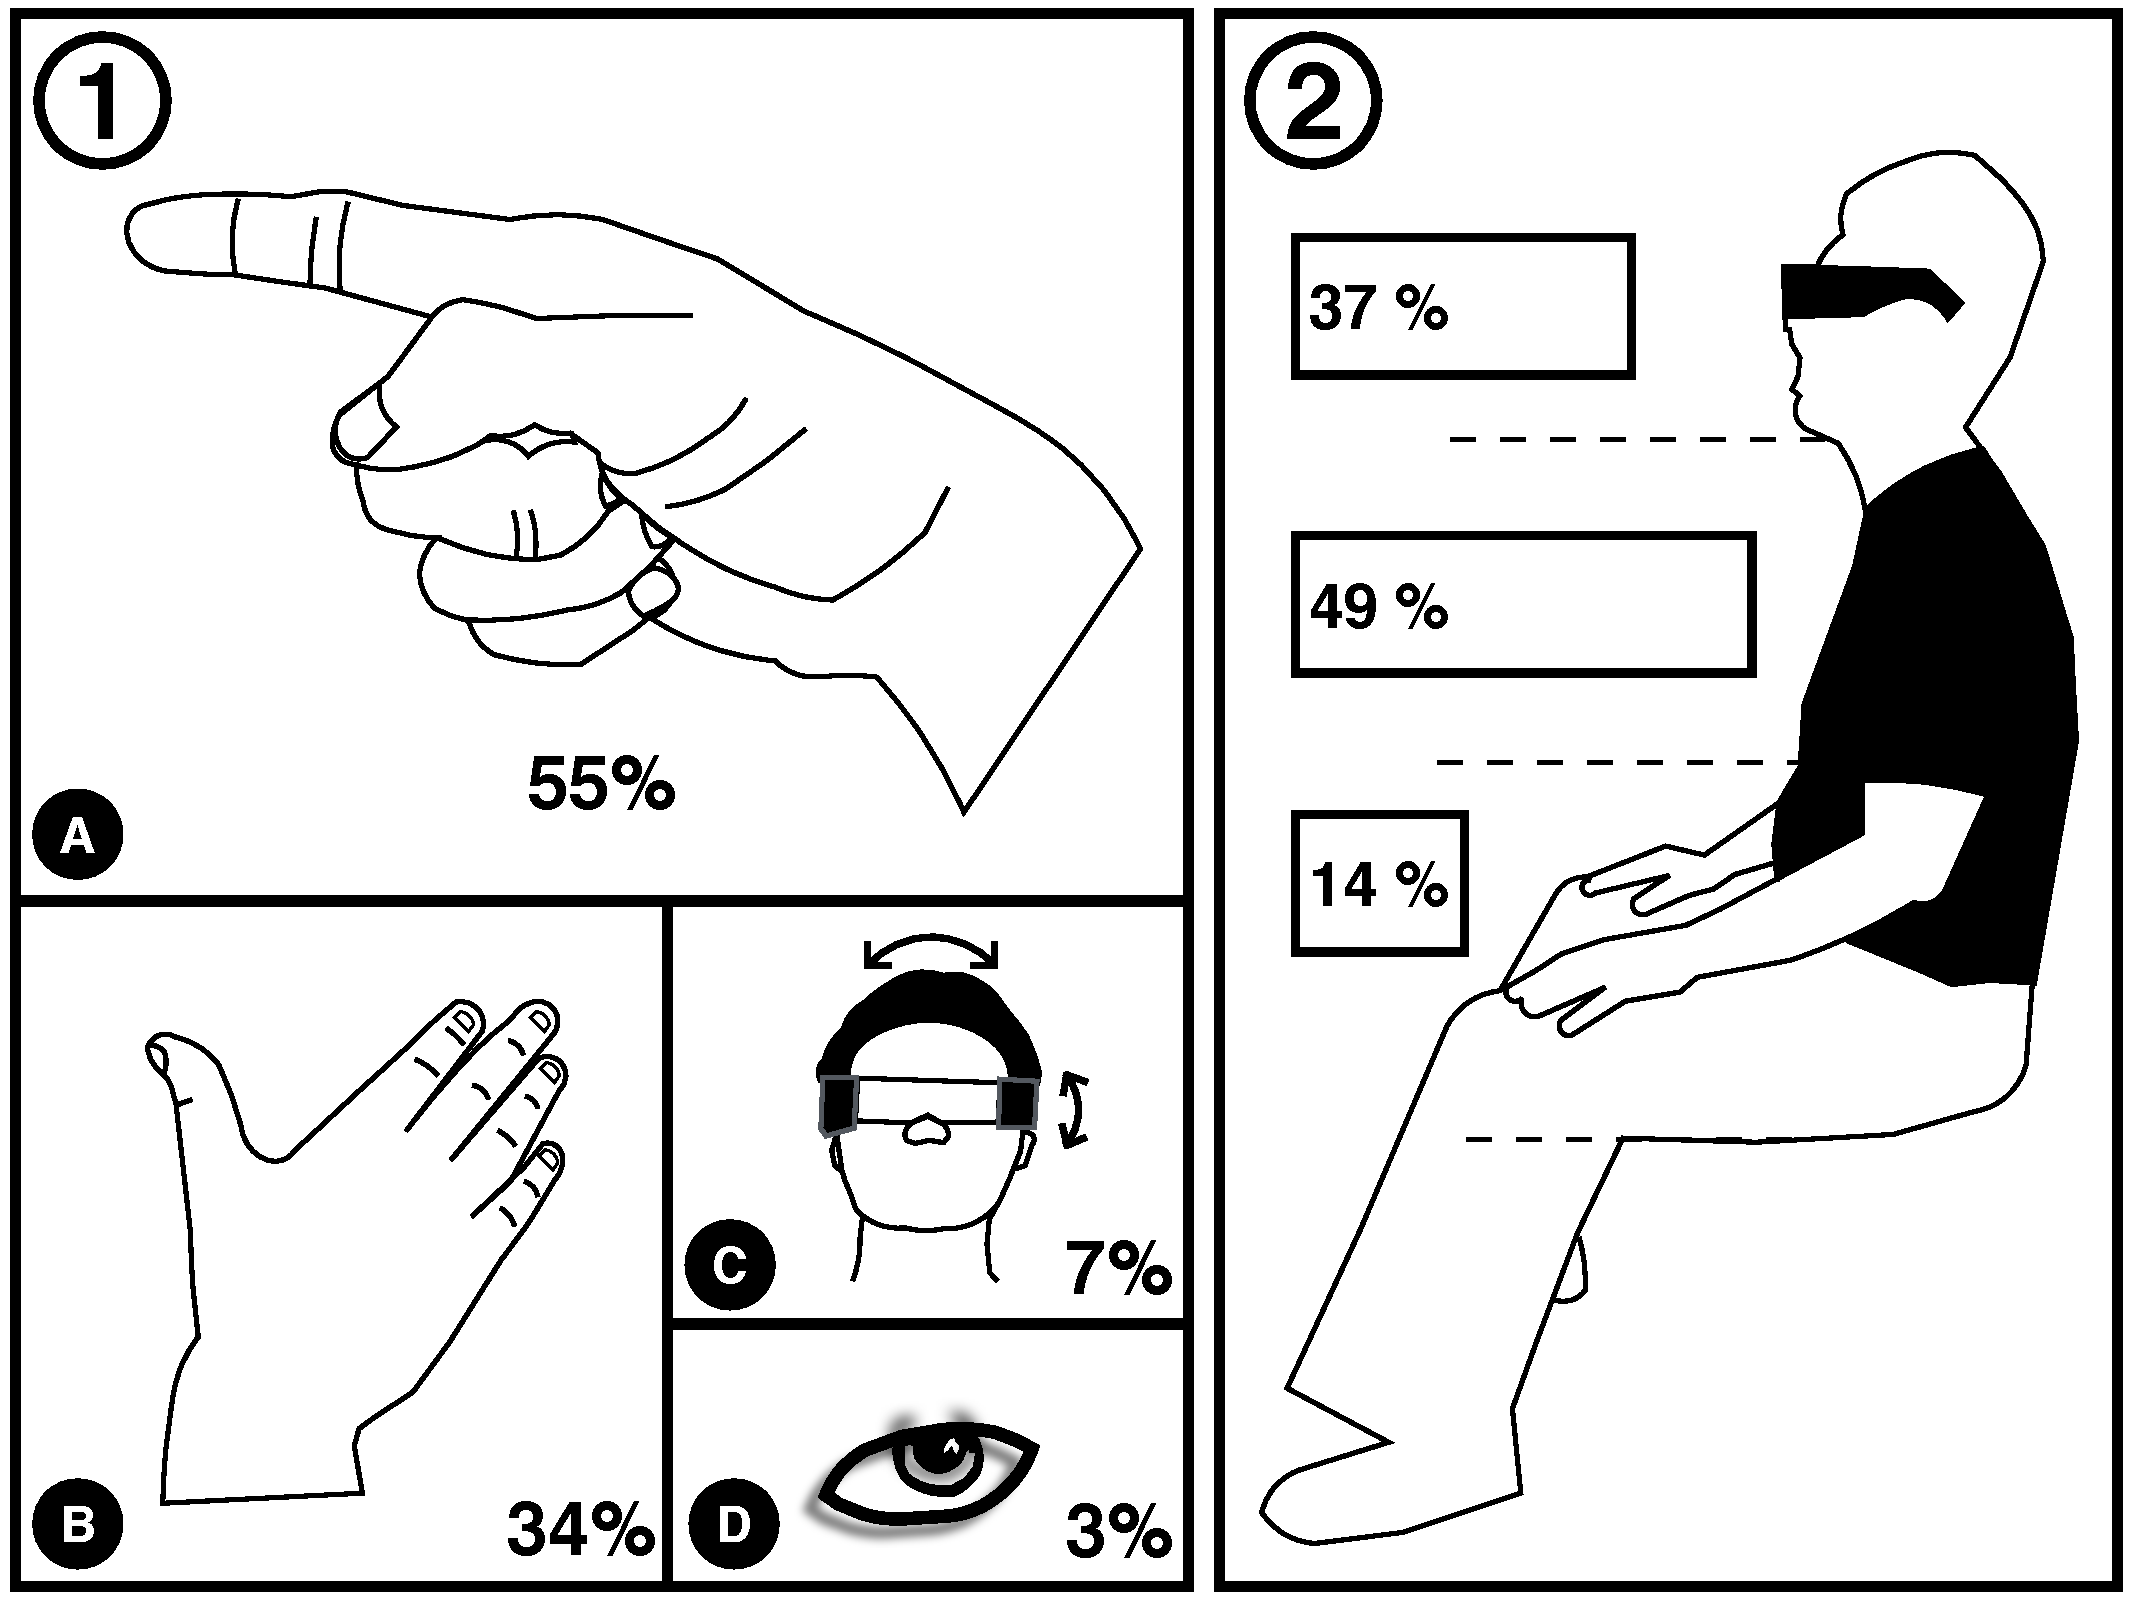
\includegraphics[width=0.8\columnwidth]{Figures/InAirControlArea}
  \caption{1.The top 4 \emph{non-touch} interaction forms. Percentages indicate the portion of \emph{non-touch} game inputs that consisted of the pictured input. (A)Using a finger to perform an in-air gesture. (B)Using the full hand to perform an in-air gesture. (C)Using head-tilting to perform game input. (D)Using eye-gestures to perform game input. 2.The distribution of the in-air gesture input area. Half of the in-air gestures (49\%) were performed in front of the chest, 14\% in front of or below the belly, and only 37\% of the gestures were performed in front of the face.}
  \label{fig:figureInAirPorpotion}
  \end{figure}


  \section{Implications for Game Design}
  According to the agreement scores we found that, no matter if using \emph{touch} interaction or \emph{non-touch} input, the average agreement between users was only .26, and the highest agreement was just about .55 (see Figure \ref{fig:Agreement}). In this case, guessing the game inputs would become a frustrating experience for players. It indicated that game developers should design the visual guide carefully to lead users performing the input action, or show an instruction to explain the input methods.

  \section{Contribution to non-gaming scenarios}
  When we first set out to explore interaction design for smart glasses, we focused on a specific domain in order to gain deeper insight and to keep the study tractable. Looking back at the results, some the study findings do apply to non-gaming scenarios. For example, many of our tasks are also used in non-gaming applications, such as ``Select single from many'', ``Vertical menu'', ``Horizontal menu'', ``Move left and right'', ``Move in 4 directions'', ``Move object to position'', ``Draw a path'' and ``Rotate an object''. Also, study results showed several facts that are useful for general cases: (1) Social acceptance of input is a significant concern in public space; (2) Performing in-air gestures in front of the face is weird and not socially acceptable; (3) If the input surface does not have an influence on the meaning of the gestures, users prefer to perform the gestures on a surface reached with least movement.
  \section{Limitation and Next Steps}



  As we know, there are many different places known as public space, and users may behave differently in each specific place. Furthermore, in our study, we did not ask users to define any input actions to interact with tangible objects in public space, such as, tables or chairs in the cafe shop. We only made participants experience two types of smart glasses. Therefore, our user-defined game input set might not be suitable to be applied to games on other types of head-worn devices. Moreover, our participants were all literate Taiwanese adults; undoubtedly, children, elders, participants from other cultures, or uneducated participants would behave differently. That is to say, these issues are worthy of investigation, but exceed the range of our current work.

  An important next step is to validate our user-defined game input set with a wearable system, which can sense all \emph{touch} and \emph{non-touch} input actions listed in our set.   
